\section{Método de Gauss-Seidel}

O método de Gauss-Seidel consiste em uma evolução algébrica direta do paradigma iterativo estabelecido por Gauss-Jacobi. A priori, a metodologia busca determinar a solução de um sistema $Ax = b$ substituindo as aproximações do vetor simultaneamente durante a própria iteração contínua. Em vez de congelar todo o vetor de estado no instante $k$ para calcular o estado $k+1$, o método de Gauss-Seidel utiliza as variáveis recém-calculadas assim que se tornam disponíveis. Dessa forma, o algoritmo otimiza o fluxo de propagação de informações através da matriz, induzindo, para a grande maioria das topologias bem comportadas, uma taxa de convergência notavelmente superior.

\subsection{Fundamentação Teórica}

O desenvolvimento matemático do método repousa na separação espectral da matriz de coeficientes $A = D - L - U$. No entanto, diferentemente da formulação anterior, a lei de recorrência agrupa a matriz inferior $L$ (onde residem as variáveis já computadas na iteração corrente) com a matriz diagonal $D$. A formulação analítica do sistema iterativo é deduzida da relação algébrica:

\begin{equation}
    (D - L)x^{(k+1)} = b + U x^{(k)} \implies x^{(k+1)} = (D - L)^{-1} b + (D - L)^{-1} U x^{(k)}
\end{equation}

Em termos práticos de somatória elementar para cada linha $i$, torna-se evidente que a parcela dependente das variáveis $x_1, \dots, x_{i-1}$ referencia o estado evoluído $k+1$, enquanto a parcela $x_{i+1}, \dots, x_n$ referencia o estado defasado $k$:

\begin{equation}
    x_i^{(k+1)} = \frac{1}{a_{ii}} \left( b_i - \sum_{j=1}^{i-1} a_{ij} x_j^{(k+1)} - \sum_{j=i+1}^{n} a_{ij} x_j^{(k)} \right)
\end{equation}

As condições de convergência são ditadas pelo raio espectral da matriz de transição $T_{GS} = (D - L)^{-1} U$. A convergência global assintótica é rigorosamente garantida se a matriz $A$ for estritamente diagonalmente dominante, simétrica positiva definida, ou se obedecer ao Critério de Sassenfeld, onde os coeficientes de ponderação $\beta_i$ devem atestar um máximo $\max(\beta_i) < 1$. Por mais que a ordem do erro seja de caráter empírico linear, na norma geral, a constante subjacente à atenuação do erro torna-se inferior à obtida pelo método de Jacobi.

\subsection{Estratégia de Implementação}

A arquitetura do método elimina a dualidade de alocação temporal. A reatribuição \textit{in-place} é natural em Python, uma vez que a sobrescrita das variáveis na mesma lista desencadeia o efeito dominó imposto pela fórmula analítica do método.

\begin{lstlisting}[language=Python, caption={Algoritmo Resumido In-Place de Gauss-Seidel}, label={lst:gauss_seidel}]
def gauss_seidel(A, b, tol=1e-5, max_iter=100, x0=None):
    n = len(A)
    x = list(x0) if x0 else[0.0 for _ in range(n)]
    
    for iteracao in range(1, max_iter + 1):
        x_ant = list(x)
        
        for i in range(n):
            soma = sum(A[i][j] * x[j] for j in range(n) if j != i)
            if abs(A[i][i]) == 0.0:
                raise ValueError(f"Pivot nulo encontrado na linha {i}.")
            x[i] = (b[i] - soma) / A[i][i]
            
        max_diff = max(abs(x[i] - x_ant[i]) for i in range(n))
        max_x = max(abs(v) for v in x)
        erro = max_diff / max_x if max_x != 0 else max_diff
        
        if erro < tol:
            return x, iteracao
            
\end{lstlisting}

Justifica-se a abordagem contígua (\texttt{soma = sum(A[i][j] * x[j] ...)}) pois o referenciamento ao iterável \texttt{x[j]} capta os índices $j < i$ naturalmente já recalculados no laço corrente. A persistência isolada de \texttt{x\_ant} serve unicamente à determinação da norma infinito para o critério de tolerância $\epsilon$. O encerramento condicional ocorre sem comprometer a estrutura temporal da matriz original.

\subsection{Estrutura dos Arquivos de Entrada e Saída}

Seguindo o paradigma modular consolidado, a malha de hiperparâmetros (vetor inicial, limites) reside em arquivos vetoriais. Notavelmente, a gravação de saídas deste método condensa vetores sucessivos numa planilha (\texttt{.csv}). Os registros mostram variações residuais acentuadas logo nas fases embrionárias, demonstrando um refinamento superior na primeira metade do ciclo temporal, cuja interpretação é delegada ao documento base por via dos scripts de diagramação subjacentes.

\subsection{Problemas Teste}

\subsubsection{Problema Teste 1: Comparativo de Redução Espectral}

O sistema selecionado foi idêntico ao modelo avaliado no método antecedente, assegurando uma base metodológica justa para atestar a redução do esforço computacional:

\begin{equation}
\begin{bmatrix}
10.00 & 2.00 & 1.00 \\
1.00 & 5.00 & 1.00 \\
2.00 & 3.00 & 10.00
\end{bmatrix}
\begin{bmatrix}
x_1 \\
x_2 \\
x_3
\end{bmatrix}
=
\begin{bmatrix}
7.00 \\
-8.00 \\
6.00
\end{bmatrix}
\end{equation}

Submetido à restrição vetorial de início estático nulo, os registros logarítmicos capturaram um comportamento agressivo de anulação do erro escalar:

\begin{table}[h]
\centering
\caption{Histórico Iterativo do Erro em Gauss-Seidel (Problema 1)}
\label{tab:seidel_prob1}
\begin{tabular}{cccc}
\hline
\textbf{Iteração ($k$)} & \textbf{Vetor Atualizado Sequencialmente} & \textbf{Deslocamento ($\Delta x$)} & \textbf{Erro Relativo} \\ \hline
1 & $[0.700, -1.740, 0.982]^T$ & 1.740 & 1.0000 \\ 
2 & $[0.949, -1.986, 1.005]^T$ & 0.249 & 0.1256 \\ 
3 & $[0.996, -2.000, 1.000]^T$ & 0.046 & 0.0234 \\
7 & $[1.000, -2.000, 1.000]^T$ & 0.000007 & 0.000003 \\ \hline
\end{tabular}
\end{table}

A análise contígua da Tabela \ref{tab:seidel_prob1} atesta uma compressão considerável no tempo da rotina. Observa-se que, ao alavancar o valor recém extraído de $x_1^{(1)} = 0.700$ para calcular $x_2^{(1)}$, o polinômio já incluiu parte da topologia da solução. Como efeito direto, o método necessitou de apenas 7 iterações para atingir a ordem restritiva de $10^{-5}$, quase a metade do custo frente a Gauss-Jacobi. O resíduo vetorizado provou, após a substituição regressiva no hiperplano matricial, tendendo ao zero absoluto.

A topologia do declínio temporal atesta a sensibilidade superior, com uma constante angular perceptivelmente mais vertical:

\begin{center}
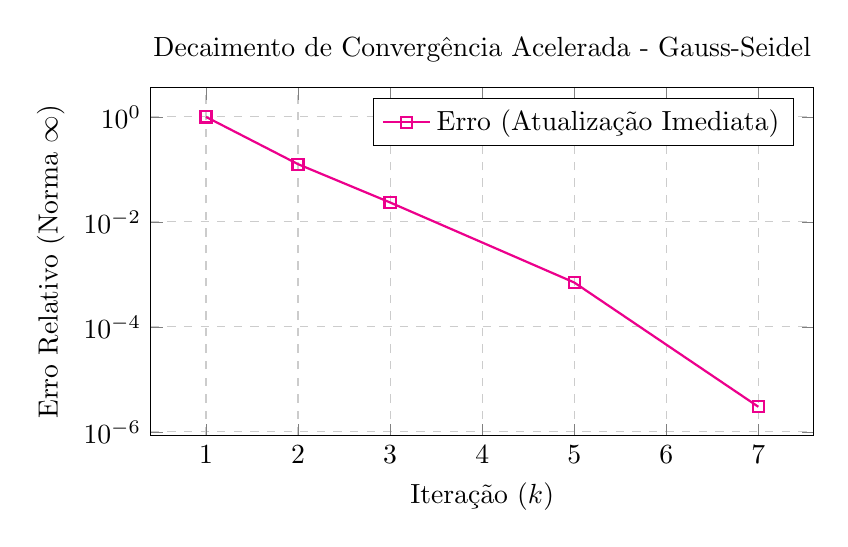
\begin{tikzpicture}
\begin{axis}[
    width=10cm, height=6.0cm,
    ymode=log,
    xlabel={Iteração ($k$)},
    ylabel={Erro Relativo (Norma $\infty$)},
    grid=major,
    grid style={dashed, gray!40},
    title={Decaimento de Convergência Acelerada - Gauss-Seidel},
    legend pos=north east
]
\addplot[
    color=magenta,
    mark=square,
    thick
] coordinates {
    (1, 1.0)
    (2, 0.1256)
    (3, 0.0234)
    (5, 0.0007)
    (7, 0.000003)
};
\addlegendentry{Erro (Atualização Imediata)}
\end{axis}
\end{tikzpicture}
\end{center}

\subsection{Dificuldades Enfrentadas}

A síntese crítica de desempenho identificou que as vantagens inerentes a Seidel implicam perdas agudas na escalabilidade contemporânea. Diferentemente do Jacobi, o método não pode ser decomposto linearmente para processos massivamente paralelos (GPGPU), já que a iteração em $x_i$ depende imperativamente que a \textit{thread} responsável por $x_{i-1}$ termine sua execução. Dessa forma, observa-se ainda que em estruturas mal condicionadas limítrofes, a injeção imediata de um salto espúrio em $x_1$ induz um efeito chicote desestabilizando todos os valores decorrentes da mesma iteração, ampliando transitoriamente as flutuações antes que a restrição de Sassenfeld possa reordenar o trajeto contínuo.